\setcounter{part}{14}  % F

\part{Mécanique des fluides}
%%%% Nombres sans dimension définis dans physics2.sty
% \ReN Reynolds
% \RoN Rossby

\section{Statique des fluides}
% Niveau :      PCSI
% Discipline :  Mécaflu
%Mots clés :    

\begin{exercise}{Fréquence de Brunt--Väisälä}{2}{Sup, Spé}
{Statique des fluides}{bermu}

Dans cet exercice, on considère un fluide dit stratifié, ayant des profils de densité et de pression $\rho(z)$, $P(z)$, $z$ étant l'altitude, sous un profil de gravité uniforme $\vec{g} = -g\ve_z$. On étudie la dynamique d'un petit cube de taille $a$ de ce fluide, dont on repère l'altitude par la variable $\xi$.

\begin{questions}
    \questioncours \'Etablir l'équation différentielle vérifiée par $\xi$ et redémontrer l'équation de la statique des fluides. 
    \uplevel{On suppose par la suite que le fluide est globalement à l'équilibre hydrostatique.
    
    Le cube, initialement à l'altitude $\xi = 0$ et de densité $\rho(0) = \rho_0$, est élevé à une altitude $\xi > 0$, sans dilatation.}
    \question \'Etablir l'équation différentielle vérifiée par $\xi$. Quelle forme classique prend-t-elle ? Montrer que suivant une condition sur $\dv{\rho}{z}$, la stratification du fluide est stable, ou instable.
    \question Quel est le comportement du cube dans le cas d'une stratification stable ? Introduire une fréquence typique, notée $N$, la fréquence de Brunt--Väisälä. 
    \begin{EnvUplevel} On se propose d'étudier un tel exemple avec la photographie suivante :
    \begin{figure}[H]
        \centering
        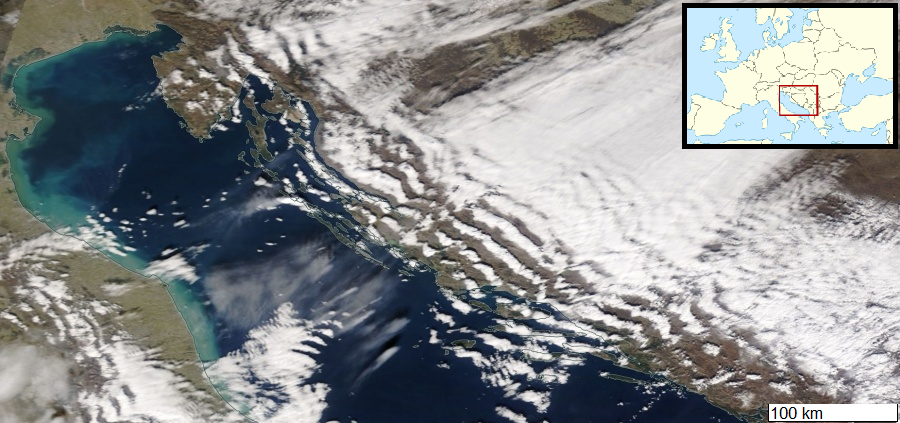
\includegraphics[width=\linewidth]{mecaflu/statiqueflu/gravity_waves.png}
        \caption{Ondes internes photographiées au large de la mer Adriatique le 25/02/2019. \newline Elles sont formées par la rencontre d'un courant d'air de haute altitude avec les Alpes dinariques dans les Balkans (Slovénie, Croatie, Bosnie, Serbie...)}
    \end{figure}
    \end{EnvUplevel}
    \question Estimer la longueur d'onde de cette onde. En déduire à l'aide des données météorologiques la fréquence associée.
    \question En utilisant la relation des gaz parfaits, en déduire une estimation du gradient thermique $\dv{T}{z}$ en $\SI{}{K/km}$.
\end{questions}

\paragraph{Données :}
\begin{itemize}
    \item accélération de la pesanteur terrestre $g = 9,81$ m$^2\cdot$s$^{-1}$,
    \item constante des gaz parfaits $R = 8,314$ $\mathrm{J\cdot mol^{-1}\cdot m^{-3}}$,
    \item pour l'air $M = 28,9$ g$\cdot$mol$^{-1}$
    \item extrait du bulletin météorologique marine du 25/02/2019 dans l'Adriatique nord : \\
    \texttt{VENTS : haute altitude ($> \SI{3000}{m}$), Nord-Est, 60 noeuds ($\SI{30}{m/s}$), température $\SI{297}{K}$.}

\end{itemize}
\end{exercise}

\begin{solution}

\begin{questions}
    \questioncours Bilan des forces : gravité $-\rho(\xi) a^3 g$, pression : $a^2 \qty\big(P(\xi-a/2) - P(\xi+a/2)) \simeq -a^3\eval{\dv{P}{z}}_\xi $. Ainsi
    $$\rho(\xi) \ddot{\xi} = - \rho(\xi) g - \eval{\dv{P}{z}}_\xi \qqtext{soit en statique} \pdv{P}{z} = -\rho g$$
    \question Ainsi en pas statique
    $$\rho(0) \ddot{\xi} = - \rho(0) g - \eval{\dv{P}{z}}_\xi = g\qty\big(\rho(\xi) - \rho(0)) \simeq g \dv{\rho}{z} \xi$$
    soit
    $$\ddot{\xi} -\dfrac{g}{\rho_0}\dv{\rho}{z}\xi = 0$$
    On a une équation d'oscillateur harmonique si $\dv{\rho}{z} < 0$ $=$ stratifié stable, le mouvement oscille. Sinon on diverge.
    \question Le cube oscille à une fréquence $N = \sqrt{-\dfrac{g}{\rho_0}\dv{\rho}{z}}$
    \question $\lambda = \SI{16}{km}$. Ainsi si $v =\SI{30}{m/s}$, $f = v/\lambda = \SI{2e-3}{s^{-1}}$
    \question $N^2 = -\dfrac{g}{\rho_0}\dv{\rho}{z}$ et $P_0 M = \rho R T_0$ donne $N^2 = -\dfrac{g}{T_0}\dv{T}{z}$. Donc $\dv{T}{z} = \SI{0.1}{K/km}$.
\end{questions}

Plus : \url{https://www.atmos.millersville.edu/~adecaria/ESCI342/ANSWERS/esci342_exercises_answers_lesson09.html}

\end{solution}
% Niveau :      PCSI
% Discipline :  Mécaflu
%Mots clés :    

\begin{exercise}{Le profil de la tour Eiffel}{1}{Sup, Spé}
{Statique des fluides, Mécanique}{bermu}

\begin{questions}
    \questioncours Redémontrer l'équation de la statique des fluides. 
\begin{EnvUplevel}
Dans ce qui va suivre, on s'intéresse au profil de la tour Eiffel.
\begin{figure}[H]
    \centering
    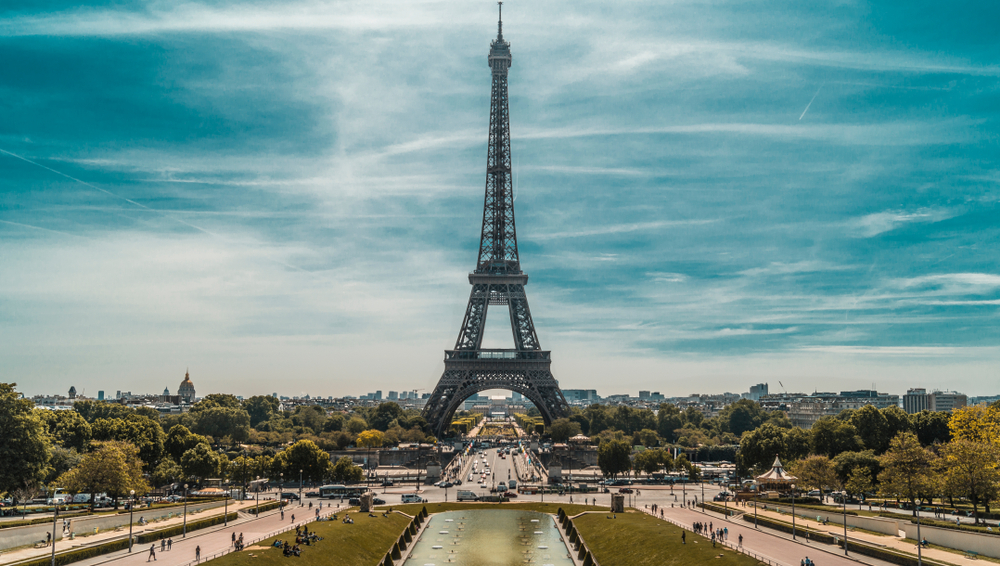
\includegraphics[width=\linewidth]{mecaflu/statiqueflu/eiffel.png}
    \vspace{-1.5em}
    \caption{La tour Eiffel depuis le Trocadéro.}
\end{figure}
\end{EnvUplevel}
    \question Considérant que la structure de la tour Eiffel est conçue afin que chaque étage exerce la même pression sur les étages inférieurs (on pourra discuter de ce principe d'ingénierie civile), établir à l'aide de la figure ci-dessus et des données un modèle simple de la tour Eiffel et donner alors l'équation de son profil.
\end{questions}

\paragraph{Données :}
\begin{itemize}
    \item accélération de la pesanteur terrestre $g = 10$ m$^2\cdot$s$^{-1}$,
    \item masse volumique de l'acier $\rho = 8\cdot 10^3$ $\mathrm{kg\cdot m^{-3}}$,
    \item hauteur de la tour Eiffel $H = 300$ m,
    \item largeur de la base de la tour Eiffel $L = 125$ m.
\end{itemize}
\end{exercise}
% Niveau :      PCSI
% Discipline :  Mécaflu
%Mots clés :    

\begin{exercise}{Le barrage de Cap de Long}{1}{Sup, Spé}
{Statique des fluides, Mécanique, Moment cinétique}{bermu}

\begin{questions}
    \questioncours Redémontrer l'équation de la statique des fluides et donner l'expression de la pression dans une retenue d'eau en fonction de la profondeur $z$. 
\begin{EnvUplevel}
Dans ce qui va suivre, on s'intéresse à comment construire un barrage tout en évitant la catastrophe. Il existe deux grands types de barrages, les barrages poids et les barrages voûte :
\begin{figure}[H]
    \centering
    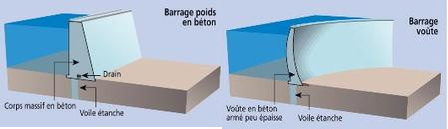
\includegraphics[width=\linewidth]{mecaflu/statiqueflu/capdelong1.png}
    \vspace{-2em}
    \caption{Les deux familles de barrages : barrage poids et barrage voûte.}
\end{figure}
\end{EnvUplevel}
    \question Commençons par étudier un barrage poids, de hauteur $H$, et d'épaisseur au sol $\ell$.
\begin{parts}
    \part Justifier qualitativement la forme du barrage.
    \part Modéliser la force totale qui s'applique sur la paroi du barrage (on prêtera attention au traitement de la pression atmosphérique). \\
    Application numérique, à mettre en perspective avec des ordres de grandeur connus. \label{que:forcetot}
    \part Exprimer la condition d'équilibre du barrage et donner une condition sur l'épaisseur maximale au sol et la hauteur.
    \part Évaluer la force exercée par le sol sur le barrage nécessaire pour que celui-ci ne soit pas emporté. Mettre ce résultat en perspective avec celui de la question \ref{que:forcetot}
\end{parts}

    \question Continuons avec un barrage voûte, de hauteur $H$, de rayon de courbure $R_\textsc{c}$ et d'épaisseur $\ell$.
\begin{parts}
    \part Quelle est qualitativement la différence avec la configuration précédente. Quels avantages ou inconvénients ?
    \part La force totale qui s'applique sur la paroi du barrage est-elle sensible à la géométrie du barrage ?
    \part Évaluer la force exercée par le sol \underline{et les contreforts} sur le barrage nécessaire pour que celui-ci ne soit pas emporté. Comparer avec les résultats de la question précédente.
\end{parts}
\end{questions}

\begin{wrapfigure}{l}{0.55\textwidth}
    \centering
    \vspace{-1em}
    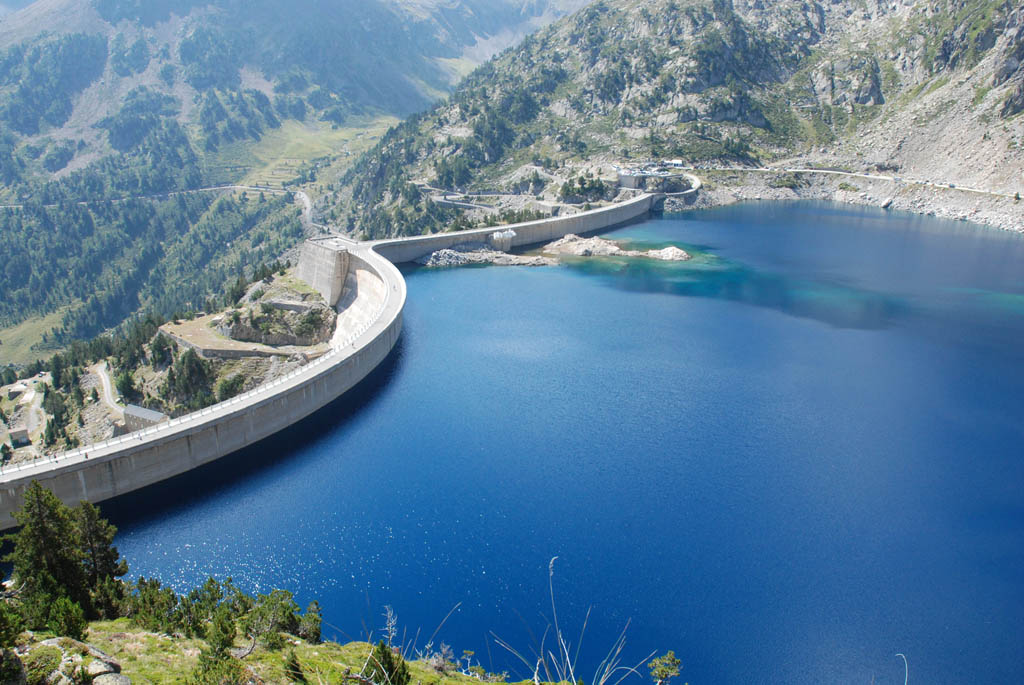
\includegraphics[width=0.8\linewidth]{mecaflu/statiqueflu/capdelong2.png}
    \vspace{-1em}
    \caption{Le barrage de Cap de Long, 101 m de haut, est la plus grande retenue d'eau des Pyrénées.}
\end{wrapfigure}


\paragraph{Données :}
\begin{itemize}
    \item pesanteur terrestre $g = 10$ m$^2\cdot$s$^{-1}$,
    \item densité du béton armé $d= 3,5$.
\end{itemize}
\end{exercise}
% Niveau :      PCSI
% Discipline :  Mécaflu
%Mots clés :    

\begin{exercise}{Atmosphère polytropique}{2}{Sup, Spé}
{Statique des fluides, Thermodynamique}{bermu}

\begin{questions}
    \questioncours Redémontrer l'équation de la statique des fluides. 
\uplevel{Dans ce qui va suivre, on s'intéresse à modéliser l'atmosphère de manière réaliste.}    
    \question Considérant que l'atmosphère est un gaz parfait avec un profil température constant $T_0$, exprimer le profil de pression $P(z)$ en fonction de l'altitude $z$ et d'une échelle caractéristique de longueur $H$, dont on donnera l'expression, la valeur et le sens physique.
    \question Comparer ce profil avec les données.
    \question Considérant les données météorologiques, proposer un modèle plus réaliste pour la troposphère et déduire une nouvelle expression de $P(z)$. Comparer avec le profil précédent.
\begin{EnvUplevel}
La \emph{loi polytropique} d'indice $k$ lie la pression du gaz et sa masse volumique $\mu$ comme
$$P = \text{cte}\times\mu^k.$$
\end{EnvUplevel}
    \question Que signifie $k = 0$ ? $k = 1$ ? $k = \gamma$ ? $k = +\infty$ ?
    \question En supposant que l'atmosphère est $k$-polytropique, calculer le profil de pression $P(z)$ et de température $T(z)$.
    \question Quelle valeur de $k$ vous semble pertinente pour modéliser la troposhère ? La stratosphère ? La mésosphère ? \\
    Quelles sont les limites de ce modèle ?
    \questionbonus Donner au moins une raison pour laquelle le modèle de l'atmosphère polytropique n'est valide que pour des intervalles restreints d'altitude ?
\end{questions}

\paragraph{Données :}
\begin{itemize}
    \item accélération de la pesanteur terrestre $g = 9,81$ m$^2\cdot$s$^{-1}$,
    \item constante des gaz parfaits $R = 8,314$ $\mathrm{J\cdot mol^{-1}\cdot m^{-3}}$,
    \item pour l'air $M = 28,9$ g$\cdot$mol$^{-1}$, $\gamma = 1,40$,
    \item données météorologiques : \\
\quad à l'altitude $z=0$ km, $T_0=300$ K, $P_0 = 10^5$ Pa.

\begin{figure}[H]
    \centering
    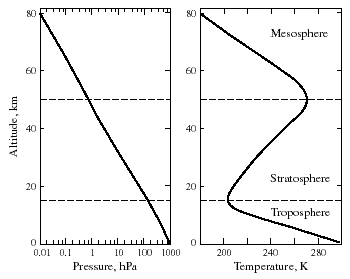
\includegraphics[scale=.85]{mecaflu/statiqueflu/polytrope.png}
    \vspace{-1.5em}
    \caption{Profils atmosphériques de pression et de température en fonction de l'altitude.}
\end{figure}
\end{itemize}
\end{exercise}
% Niveau :      PC
% Discipline :  Mécaflu
%Mots clés :    Parallèle Equations de Maxwell et gravité

\begin{exercise}{Mesure du nombre d'Avogradro}{2}{Spé}
{Statique des fluides, Thermodynamique}{bermu}

\begin{questions}
    \questioncours\label{que:perrin} Redémontrer l'équation de la statique des fluides.
    \questionbonus Contribution scientifiques de Jean Perrin.
\begin{EnvUplevel}
En 1913, Jean Perrin publie \emph{Les Atomes}, ouvrage dans lequel il entend imposer une fois pour toutes par un argumentaire fourni l'hypothèse atomique. Parmi ces preuves, il étudie la répartition à l'équilibre de '\emph{grains}' dans une émulsion, qu'il compte au microscope, afin de calculer le nombre d'Avogadro. Voici ses observations :

\begin{center}\begin{minipage}{155mm}
    «\itshape On constate que \emph{[peu après l'agitation]} les couches inférieures deviennent  plus  riches  en grains  que  les  couches  supérieures,  mais  que  cet  enrichissement  se ralentit sans cesse, et que l’aspect de l’émulsion finit par ne plus changer. Il se réalise bien un état de régime permanent dans lequel la concentration décroît avec la hauteur. \normalfont »
\end{minipage}\end{center}
\end{EnvUplevel}
    \question Interpréter qualitativement ces observations au regard de la question \ref{que:perrin}.
    \question Supposant que la grains se comportent à l'équilibre comme un gaz parfait (on pourra discuter de cette hypothèse), donner l'équation vérifiée par la densité $n$ (en m$^{-3}$) des grains. \\
    On fera apparaître une hauteur caractéristique $H$ qui ne dépend que des données du problème et du nombre d'Avogadro $N_\textsc{a}$.
    \question Résoudre cette équation sachant que la densité en $z = 0$ est $n_0 = 100$.
\begin{EnvUplevel}
Perrin trouve les résultats suivants :
\begin{center}\begin{minipage}{155mm}
    «\itshape Une série très soignée a été faite avec des grains de gomme ayant pour rayon 0,212~$\mu$m~\emph{[...]}.
    Des lectures croisées ont été faites dans une cuve profonde de 100 $\mu$m, en quatre plans horizontaux équidistants traversant la cuve aux niveaux
    \begin{center}
        5 $\mu$m, 35 $\mu$m, 65 $\mu$m, 95 $\mu$m.
    \end{center}
    Ces lectures ont donné pour ces niveaux \emph{[...]} des concentrations proportionnelles aux nombres :
    \begin{center}
        100 $\mu$m, 47 $\mu$m, 22.6 $\mu$m, 12 $\mu$m.
    \end{center}
    qui sont en progression géométrique. \normalfont »
\end{minipage}\end{center}\end{EnvUplevel}
    \question Le profil expérimental correspond-t-il au modèle ? \`A l'aide d'un tableur ou d'une calculatrice, donner une valeur expérimentale du nombre d'Avogadro $N_\textsc{a}$ et comparer avec la valeur standard
    $$N_\textsc{a} = 6.022\times 10^{23} \text{ mol}^{-1}.$$
\end{questions}

\plusloin
Perrin a répété cette expérience pour plusieurs valeurs de température et plusieurs types de grains, avec succès.

Malheureusement, une démonstration bien plus frappante de l'existence des atomes, les figures de diffraction par les rayons X de cristaux, sera découverte l'année suivante, rendant l'objet de son livre obsolète... 

\paragraph{Données expérimentales : } à $T = 273$ K, telles que mesurées par Perrin
\begin{itemize}
    \item masse volumique de l'eau $\rho_\mathrm{H_2O} = 1,003$ kg$\cdot$m$^{-3}$,
    \item masse volumique des grains $\rho_\text{g} = 1,194$ kg$\cdot$m$^{-3}$
    \item constante des gaz parfaits$^\dagger$ $R = 8.314$ $\mathrm{J\cdot K^{-1}\cdot mol^{-1}}$,
\end{itemize}
\medskip
$^\dagger$ \small{Elle était déjà connue à l'époque grâce aux travaux antérieurs de Clapeyron.}

\paragraph{Référence :} Jean Perrin, \emph{Les atomes}, Félix Alcan, Nouvelle collection scientifique, Paris, 1913.
\end{exercise}
% Niveau :      PC
% Discipline :  Mécaflu
%Mots clés :    Parallèle Equations de Maxwell et gravité

\begin{exercise}{Instabilité de Jeans}{3}{Spé}
{Statique des fluides, Analogie gravité--électromagnétisme}{bermu}

\begin{questions}
    \questioncours Parallèle entre le champ électrique $\vE$ et le champ gravitationnel $\vg$.
\begin{EnvUplevel}
On se place dans le vide interstellaire et on considère un nuage de poussière de géométrie sphérique de taille $R$ et de profil de densité $\rho(r)$.
\end{EnvUplevel}
    \question En utilisant le résultat précédent, donner l'expression du champ de pesanteur $\vg$ du nuage.
    \question En supposant que le nuage est à l'équilibre hydrostatique, montrer que sous certaines conditions, le nuage est instable et peut s'effondrer sur lui-même.
\end{questions}

\paragraph{Données :} en coordonnées sphériques
$$\div\vg = \dfrac{1}{r^2}\pdv{r^2 g_r}{r}.$$
\end{exercise}

\section{Bernoulli}
% Niveau :      PCSI
% Discipline :  Mécanique céleste
%Mots clés :    Astronaute

\begin{exercise}{Équilibre d'un jerrican}{2}{Sup}
{Statique des fluides}{lelay}

In étudie ici un l'équilibre d'un jerrican d'eau, c'est à dire un conteneur parallélépipèdique de hauteur $H$ et de section $A$ muni d'un petit robinet en bas et d'une grosse ouverture munie d'un bouchon en haut.
\begin{questions}
    \question On remplit le jerrican par l'ouverture du haut et on le vide par le robinet. Pourquoi est-il important de laisser le bouchon ouvert ?
    \question On suppose dans un premier temps que le jerrican est complètement rempli en eau par le bouchon, et qu'il n'y a pas d'air à l'intérieur. On ferme ensuite le bouchon.
    \begin{parts}
        \part Montrer que l'eau va couler du robinet si et seulement si la hauteur du jerrican dépasse une certaine hauteur notée $L$.
        \part Représenter le profil de pression dans le jerrican est fonction de la hauteur en considérant $H > L$
        \part Qu'y a-t-il au dessus de l'eau lorsque $H > L$ ? Quel phénomène a été négligé ?
    \end{parts}
    \question On considère maintenant que le jerrican a été rempli partiellement, et qu'un volume $V_0$ d'air se trouve à l'intérieur. On referme le bouchon et on ouvre le robinet.
    \begin{parts}
        \part Que va-t-il se passer ?
        \part À un instant quelconque $t$ il y a un volume $V_t$ d'air dans le jerrican. Quelle est la pression $P_t$ de l'air dans le jerrican ?
        \part Au bout d'un certain temps l'écoulement s'arrête. Le volume d'air est alors $V_f$ et la pression de l'air $P_f$. Exprimer l'équation d'équilibre statique en fonction de $V_f$, $L$ et de la géométrie du jerrican.
        \part Résoudre cette équation. Combien y a-t-il de solutions ? Quels sont leurs signes ? Les interpréter physiquement.
        \part A quelle condition sur $V_0$ le jerrican est-il entièrement vidé à la fin ? 
        \part Donner $V_f$ dans le cas $H = L$
    \end{parts}
\end{questions}

\end{exercise}

\begin{solution}

\begin{questions}
    \question Sinon ça coule plus au bout d'un moment.
    \question On suppose dans un premier temps que le jerrican est complètement rempli en eau par le bouchon, et qu'il n'y a pas d'air à l'intérieur. On ferme ensuite le bouchon.
    \begin{parts}
        \part Statique des fluides de base, c'est l'expérience de torricelli, $L = P_0/\rho g$
        \part zéro en haut, et ça croit linéairement de $0$ à $P_0$ avec une pente $\rho g$
        \part Du vide, mais on a négligé le fait qu'à basse pression l'eau change d'état donc c'est pas strictement du vide.
    \end{parts}
    \question On considère maintenant que le jerrican a été rempli partiellement, et qu'un volume $V_0$ d'air se trouve à l'intérieur. On referme le bouchon et on ouvre le robinet.
    \begin{parts}
        \part Ca va couler puis s'arrêter
        \part $P_t = P_0 \frac{V_0}{V_t}$, loi de Boyle-Mariotte
        \part $\frac{V_f^2}{L} + \qty(1-\frac{H}{L}) V_f - V_0 =0$
        \part Équation du second degré au déterminant positif : 2 solutions. Une toujours positive : c'est celle qu'on cherche. Une toujours négative : Elle utilise des volumes négatifs et des pressions négatives, elle n'est donc pas physique.
        \part Jerrican vidé a la fin : $V_f > AH$. On trouve $V_0 > AH$, donc ça n'arrive jamais
        \part C'est $\sqrt{V_0 A H}$
    \end{parts}
\end{questions}

\end{solution}

\section{Tension superficielle}
% Niveau :      PC
% Discipline :  Mécaflu
%Mots clés :    Tension superficielle

\begin{exercise}{Ascension capillaire}{2}{Spé}
{Statique des fluides, Tension superficielle, Capillarité}{bermu}

\begin{questions}
    \questioncours Rappeler ce que sont les effets de tension de surface et les modéliser rapidement. On définira le coefficient de tension de surface $\gamma$.
\begin{EnvUplevel}
\paragraph{Rappel :} loi de Laplace \\
\`A l'interface entre deux fluides $a$ et $b$ non miscibles, la tension de surface (dont le coefficient est $\gamma_{ab}$) créée une surpression telle que
$$P_b - P_a = \dfrac{2\gamma_{ab}}{R_c},$$
$R_c$ étant le rayon de courbure de l'interface.

\begin{multicols}{2}
\begin{figure}[H]
    \centering
    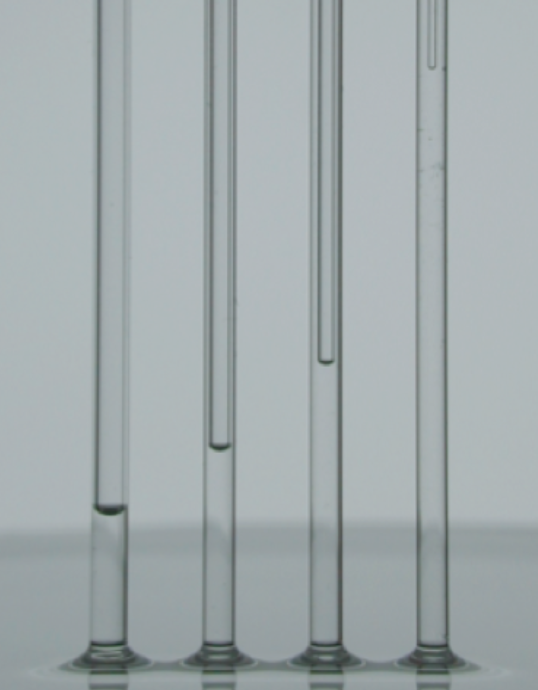
\includegraphics[width=\linewidth]{mecaflu/jurin1.png}
    \vspace{-1em}
    \caption{Ascension capillaire dans des tubes de différentes tailles.}\label{fig:jur1}
\end{figure}
\begin{figure}[H]
    \centering
    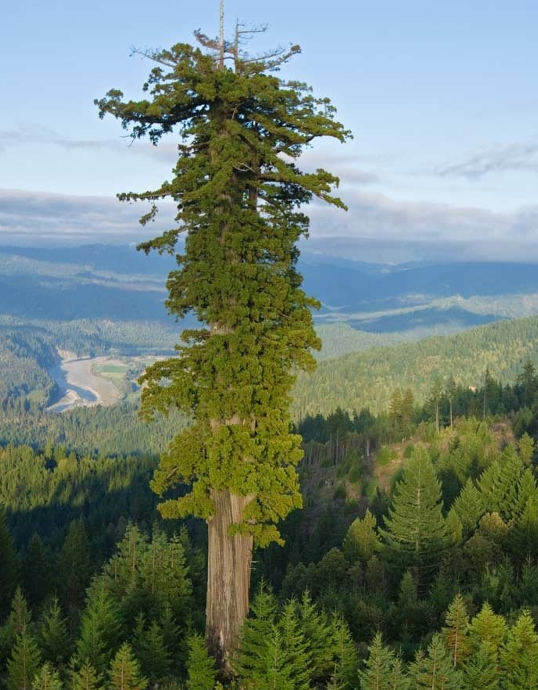
\includegraphics[width=\linewidth]{mecaflu/jurin2.png}
    \vspace{-1em}
    \caption{\emph{Hypérion}, l'arbre le plus haut du monde.}\label{fig:jur2}
\end{figure}
\end{multicols}

\end{EnvUplevel}
    \question \`A l'aide de la loi de Laplace, expliquer la figure \ref{fig:jur1} ci-dessus et estimer la tension superficielle eau--air. \\
    On appellera $\theta$ l'angle de contact entre le ménisque (que l'on supposera être une calote sphérique) et le tube.
\uplevel{L'arbre le plus haut du monde, un séquoia nommé \emph{Hypérion}  et situé dans le parc national de \emph{Redwood} en Californie (fig.~\ref{fig:jur2}), mesure 115m.}
    \question Estimer jusqu'à quelle hauteur limite la sève peut monter dans l'arbre par capillarité. \\
    Quelle peut être une autre raison de l'ascension de la sève dans les arbres ?
\end{questions}
\end{exercise}
% Niveau :      PC
% Discipline :  Mécaflu
%Mots clés :    Tension superficielle

\begin{exercise}{Ménisque et chimie}{3}{Spé}
{Statique des fluides, Tension superficielle, Capillarité}{bermu}

\begin{questions}
    \questioncours Rappeler ce que sont les effets de tension de surface et les modéliser rapidement. On définira le coefficient de tension de surface $\gamma$.
\begin{EnvUplevel}
\paragraph{Rappel :} loi de Laplace \\
\`A l'interface entre deux fluides $a$ et $b$ non miscibles, la tension de surface (dont le coefficient est $\gamma_{ab}$) créée une surpression telle que
$$P_b - P_a = \dfrac{2\gamma_{ab}}{R_c},$$
$R_c$ étant le rayon de courbure de l'interface.

\bigskip

On considère un fluide au repos en contact avec une surface solide verticale. On note $\theta$ l'angle de contact entre le fluide et la paroi.

\end{EnvUplevel}
    \question \`A l'aide de la loi de Laplace, donner l'équation de la surface libre air--fluide $z(x)$. \\
    On pourra adimensionner l'équation avec la longueur capillaire $\ell_c$ dont on donnera l'expression et le sens physique.
    \question Simplifier l'équation précédente en estimant la valeur du nombre de Bond
$$\cal{B}o = \dfrac{L}{\ell_c},$$
$L$ étant la taille typique du système.
    \question Résoudre l'équation et déduire que l'ascension de fluide typique est
$$h = \ell_c \cot\theta.$$
\end{questions}

\plusloin

En chimie, la capillarité pose souvent des problèmes pour la mesure du volume. Modéliser les erreurs typiques de mesure de volumes en chimie. Faut-il lire le volume en haut ou en bas du ménisque ?

\paragraph{Données :} rayon de courbure d'une courbe 1D $z(x)$
$$\dfrac{1}{R_c} = \dfrac{z''(x)}{\qty(1 + z'(x)^2)^{3/2}}.$$
Dans le cas d'une surface 2D ayant une symétrie de révolution $z(r)$
$$\dfrac{1}{R_c} = \dfrac{z''(r) + \frac{1}{r}\qty(1 + z'(r)^2)z'(r)}{\qty(1 + z'(r)^2)^{3/2}}.$$
\end{exercise}
% Niveau :      PC
% Discipline :  Mécaflu
%Mots clés :   Tension de surface

\begin{exercise}{Sphère flottante}{4}{Spé -- Oral X}
{Tension superficielle}{lelay}

\begin{questions}
\uplevel{On place une sphère plus dense que l'eau dans un bassin.}
    \question Trouver la relation que doivent vérifier les différents paramètres physiques en jeu pour qu'elle flotte à la moitié de sa hauteur. Cette situation est-elle stable ?

\uplevel{Maintenant, la sphère est de densité quelconque. On la jette dans l'eau depuis une certaine hauteur.}
    \question Décrire les différentes situations toujours en fonction des différents paramètres physiques en jeu.
\end{questions}
\end{exercise}

\section{\'Equations d'Euler et de Bernoulli}
% Niveau :      PCSI
% Discipline :  Mécanique céleste
%Mots clés :    Astronaute

\begin{exercise}{Équilibre d'un jerrican}{2}{Sup}
{Statique des fluides}{lelay}

In étudie ici un l'équilibre d'un jerrican d'eau, c'est à dire un conteneur parallélépipèdique de hauteur $H$ et de section $A$ muni d'un petit robinet en bas et d'une grosse ouverture munie d'un bouchon en haut.
\begin{questions}
    \question On remplit le jerrican par l'ouverture du haut et on le vide par le robinet. Pourquoi est-il important de laisser le bouchon ouvert ?
    \question On suppose dans un premier temps que le jerrican est complètement rempli en eau par le bouchon, et qu'il n'y a pas d'air à l'intérieur. On ferme ensuite le bouchon.
    \begin{parts}
        \part Montrer que l'eau va couler du robinet si et seulement si la hauteur du jerrican dépasse une certaine hauteur notée $L$.
        \part Représenter le profil de pression dans le jerrican est fonction de la hauteur en considérant $H > L$
        \part Qu'y a-t-il au dessus de l'eau lorsque $H > L$ ? Quel phénomène a été négligé ?
    \end{parts}
    \question On considère maintenant que le jerrican a été rempli partiellement, et qu'un volume $V_0$ d'air se trouve à l'intérieur. On referme le bouchon et on ouvre le robinet.
    \begin{parts}
        \part Que va-t-il se passer ?
        \part À un instant quelconque $t$ il y a un volume $V_t$ d'air dans le jerrican. Quelle est la pression $P_t$ de l'air dans le jerrican ?
        \part Au bout d'un certain temps l'écoulement s'arrête. Le volume d'air est alors $V_f$ et la pression de l'air $P_f$. Exprimer l'équation d'équilibre statique en fonction de $V_f$, $L$ et de la géométrie du jerrican.
        \part Résoudre cette équation. Combien y a-t-il de solutions ? Quels sont leurs signes ? Les interpréter physiquement.
        \part A quelle condition sur $V_0$ le jerrican est-il entièrement vidé à la fin ? 
        \part Donner $V_f$ dans le cas $H = L$
    \end{parts}
\end{questions}

\end{exercise}

\begin{solution}

\begin{questions}
    \question Sinon ça coule plus au bout d'un moment.
    \question On suppose dans un premier temps que le jerrican est complètement rempli en eau par le bouchon, et qu'il n'y a pas d'air à l'intérieur. On ferme ensuite le bouchon.
    \begin{parts}
        \part Statique des fluides de base, c'est l'expérience de torricelli, $L = P_0/\rho g$
        \part zéro en haut, et ça croit linéairement de $0$ à $P_0$ avec une pente $\rho g$
        \part Du vide, mais on a négligé le fait qu'à basse pression l'eau change d'état donc c'est pas strictement du vide.
    \end{parts}
    \question On considère maintenant que le jerrican a été rempli partiellement, et qu'un volume $V_0$ d'air se trouve à l'intérieur. On referme le bouchon et on ouvre le robinet.
    \begin{parts}
        \part Ca va couler puis s'arrêter
        \part $P_t = P_0 \frac{V_0}{V_t}$, loi de Boyle-Mariotte
        \part $\frac{V_f^2}{L} + \qty(1-\frac{H}{L}) V_f - V_0 =0$
        \part Équation du second degré au déterminant positif : 2 solutions. Une toujours positive : c'est celle qu'on cherche. Une toujours négative : Elle utilise des volumes négatifs et des pressions négatives, elle n'est donc pas physique.
        \part Jerrican vidé a la fin : $V_f > AH$. On trouve $V_0 > AH$, donc ça n'arrive jamais
        \part C'est $\sqrt{V_0 A H}$
    \end{parts}
\end{questions}

\end{solution}
% Niveau :      PC
% Discipline :  Mécaflu
%Mots clés :    Ondes de surface

\begin{exercise}{\textit{Jeux de vagues}}{3}{Spé}
{Mécanique des fluides, Fluides parfaits, Tension superficielle}{bermu}

\begin{questions}
    \questioncours Décrire et comparer à l'aide d'un tableau comportant les différents paramètres que vous jugerez pertinents (\emph{e.g.} fréquence, impédance...) les phénomènes ondulatoires physiques que vous connaissez. On conservera ce tableau pour la suite de l'exercice. \label{que:ondes}
\begin{EnvUplevel}
Nous étudions par la suite un liquide dont la surface est libre d'osciller.
\begin{figure}[H]
    \centering
    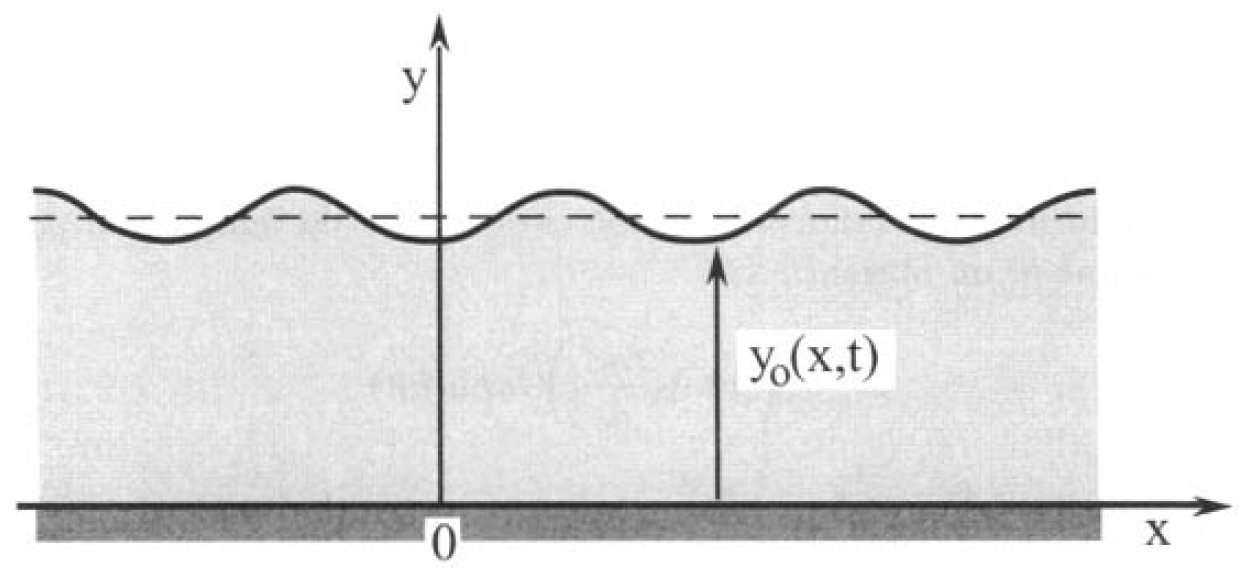
\includegraphics[width=0.5\linewidth]{mecaflu/barque.png}
    \vspace{-1.5em}
    \caption{Geometrie de la couche de liquide pour l'étude de la propagation
des ondes de surface.}
\end{figure}
Le liquide est de profondeur $h$. On supposera que les ondes sont de faible amplitude.
\end{EnvUplevel}
    \question Décrire les différents termes de l'équation d'Euler en 2D dans un champ de pesanteur $\vg$. Définir \emph{écoulement potentiel} et introduire le potentiel des vitesses $\Phi$.
    \question Montrer que dans notre cas l'équation d'Euler devient
    $$\pdv{\Phi}{t} + \dfrac{p}{\rho} + g y = \text{cte}.$$
    \question\label{que:laplace} En justifiant que l'écoulement est irrationnel et que le fluide est incompressible, montrez que $\Phi$ vérifie l'équation de Laplace.
    \question\label{que:inter} Donner les conditions aux limites pour $p$, $\Phi$ et $y_0$ en $y = y_0(x,t)$.
    \question\label{que:kelvin} En déduire que le potentiel $\Phi$ vérifie en $y = y_0(x,t)$ :
    $$\pdv[2]{\Phi}{t} + g\pdv{\Phi}{y} = 0.\vspace{-1.5em}$$
\uplevel{Nous allons à présent chercher des solutions sous forme d'onde de célérité $c$ : \  $\Phi(x,y,t) = \Phi_0 f(y) e^{ik(x-ct)}.$}
    \question Compte tenu de la question \ref{que:laplace}, donner l'expression de la fonction $f$.
    \question Déduire de la question \ref{que:kelvin} que la relation de dispersion des ondes de gravité est
    $$\omega^2 = gk\tanh(hk).$$
    Discuter de cette relation et des limites en eau peu profonde $h \ll \lambda$ et très profonde $h \gg \lambda$.
    \question Compléter le tableau de la question \ref{que:ondes} au vu de la question précédente.
\end{questions}
\plusloin[Les ondes gravito-capillaires]
La différence de pression $\Delta p$ à une interface liquide vapeur $y_0(x,t)$ ayant pour tension superficielle $\gamma$ est, pour une faible courbure de l'interface, donnée par la Loi de Laplace
$$\Delta p \simeq \gamma \pdv[2]{y_0}{x}.\vspace{-0.5em}$$
En revoyant le résultat de la question \ref{que:inter}, montrez que la relation de dispersion des ondes gravito-capillaires est\vspace*{-2ex}
$$\omega^2 = k^2 \ gh\qty(1 + \dfrac{\gamma }{\rho g}k^2)\dfrac{\tanh{kh}}{kh}.$$

\end{exercise}

\section{\'Equation de Navier--Stokes}
% Niveau :      PC
% Discipline :  Mécaflu
%Mots clés :    Viscosité vorticité

\begin{exercise}{Vorticité et aviation civile}{2}{Spé}
{Mécanique des fluides, Fluides réels}{lelay}

\begin{questions}
    \questioncours Définir les différents régimes d'écoulement dans un fluide visqueux. On donnera l'équation de Navier--Stockes et l'expression du nombre de Reynolds $\cal{R}e$.
\begin{EnvUplevel}
On défini la vorticité $\vOm$
$$\vOm = \rot\vv.$$
\end{EnvUplevel}
    \question Quel est le sens physique de la vorticité ? Quelle est l'équation de la dynamique de la vorticité ?
\uplevel{On s'intéresse à la dynamique de la vorticité autour des avions commerciaux au décollage et à l'atterrissage.}
    \question Pourquoi les avions commerciaux sont-ils séparés de quelques minutes au décollage ? Retrouver ce délai à l'aide de l'équation de la vorticité.
\end{questions}

\paragraph{Données :} quelques formules d'analyse vectorielle
\begin{align*}
    (\vv\vdot\grad)\vv &= \grad\qty(\dfrac{\vv^2}{2}) + (\rot\vv)\cross\vv \\
    \rot(\vA\cross\vB) &= (\vB\vdot\grad)\vA - (\vA\vdot\grad)\vB + \vB\,(\div\vA) - \vA\,(\div\vB)
\end{align*}
\end{exercise}
% Niveau :      PC
% Discipline :  Mécaflu
%Mots clés :    Viscosité, Couche limite, Equation de Blasius

\begin{exercise}{Couche limite visqueuse de Blasius}{3}{Spé}
{Mécanique des fluides, Fluides réels}{bermu}

\begin{questions}
    \questioncours Décrire les différents termes de l'équation de Navier--Stockes en 2D et définir le nombre de Reynolds $\ReN$. On prendra soin de la garder dans un coin du tableau pour la suite. \\
    Définir ce qu'est la \emph{couche limite} $\delta$ d'un écoulement et en donner un critère qualitatif.
\begin{EnvUplevel}
Nous étudions par la suite l'évolution du profil 2D de vitesse $\mqty(u_x \\ u_y)$ pour un écoulement de couche limite au-dessus d'une plaque plane :
\begin{figure}[H]
    \centering
    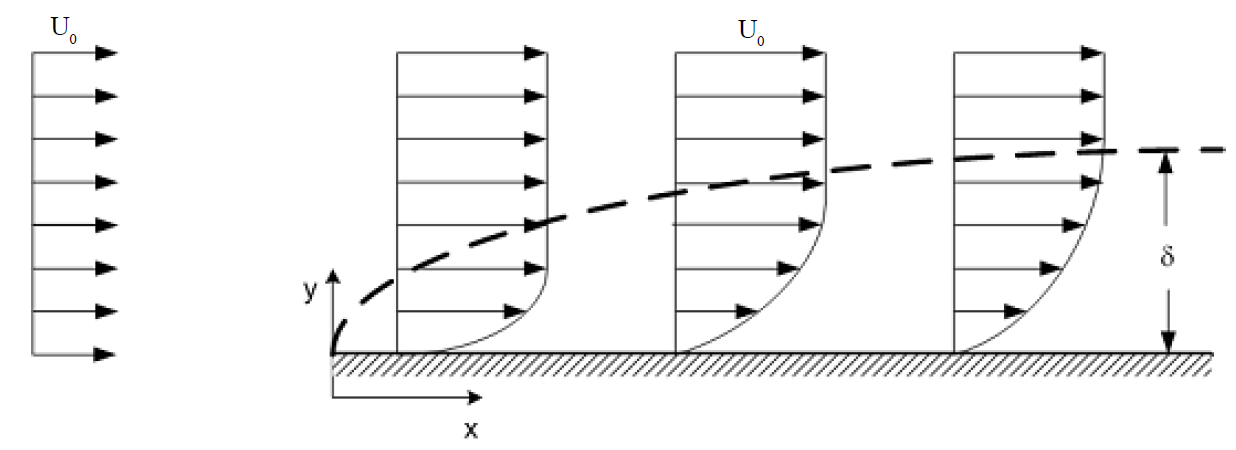
\includegraphics[width=0.8\linewidth]{mecaflu/blasius1.png}
    \vspace{-1em}
    \caption{Schéma du profil de couche limite au-dessus d'une plaque plane.}
\end{figure}
Dans ce cas, la taille de la couche limite $\delta(x)$ varie selon la distance $x$ parcourue le long de la plaque plane par le fluide.
\end{EnvUplevel}
    \question En vous aidant du schéma ci-dessus, donner les conditions aux limites pour la vitesse $u_x$, $u_y$ et la pression $p$.
\uplevel{Nous introduisons $\ReN_x$, le nombre de Reynolds ayant pour taille caractéristique $x$. Nous considérerons que la couche étudiée limite est visqueuse (par opposition à turbulente).}
    \question Quelle est l'expression de $\ReN_x$ ? Quel est son sens physique ? Est-il grand ou petit ?
    \question Justifier qualitativement que pour $y\gg\delta(x)$, les effets de viscosité sont négligeables et que par conséquent la pression y est constante $p(x,y) \simeq p_0$.
    \question Inversement, justifier qualitativement que pour $y\ll\delta(x)$, une variation de hauteur typique $\delta(x)$ peut s'écrire
    $$\delta(x) \simeq \sqrt{\dfrac{\nu x}{U_0}}.$$
    \question En utilisant le nombre de Reynolds $\ReN_x$ et le résultat précédent, justifier que
    $$\pdv{}{y} \ll \pdv{}{x},$$
    et en déduire que
    \begin{parts}
        \part la pression $p$ dans la couche limite est égale à la pression au-dessus de la couche limite ;
        \part la vitesse verticale $u_y$ ne peut pas être nulle dans la couche limite.
    \end{parts}
    \question Utilisez les résultats précédents simplifier l'équation de Navier--Stockes suivant $x$. \\
    L'équation ne comportera plus que trois termes.
    \questionbonus Cette équation peut être généralisée à n'importe quel profil d'attaque : reprendre la question précédente en prenant en compte que cette fois-ci $U_0(x)$ dépend de $x$.
\end{questions}

\begin{center}
    \itshape --- \quad Suite au verso \quad ---
\end{center}
\end{exercise}
\pagebreak

\printexerciseheader

\begin{center}
    \itshape --- \quad Suite du recto \quad ---
\end{center}

\bigskip

\begin{questions}
\setcounter{question}{8}
\question En justifiant succinctement et en utilisant le changement de variable suivant :
    $$u_x = U_0 f'(\xi), \qquad y = \xi\delta(x),$$
    montrez que l'équation de Navier--Stockes et l'équation d'incompressibilité permettent de d'obtenir l'équation de Blasius
    $$2 f'''(\xi) + f(\xi) f''(\xi) = 0.$$
    
    \textbf{Aide :} les dérivées partielles s'écrivent dans ce cas
    $$\pdv{}{x} = -\dfrac{\xi}{2x}\pdv{}{\xi} \qqtext{et} \pdv{}{y} = \dfrac{1}{\delta(x)}\pdv{}{\xi}.$$
\uplevel{L'équation de Blasius est non linéaire et ne peut être obtenue que par intégration numérique. Il faut donc trouver des conditions aux limites pour $f$.}
    \question Justifier que celles employées pour la figure ci-dessous sont
    $$f'(0) = 0,\quad f'(\infty) = 1, \quad f'''(0) = 0.$$
\begin{EnvUplevel}
La solution numérique est alors :
\begin{figure}[H]
    \centering
    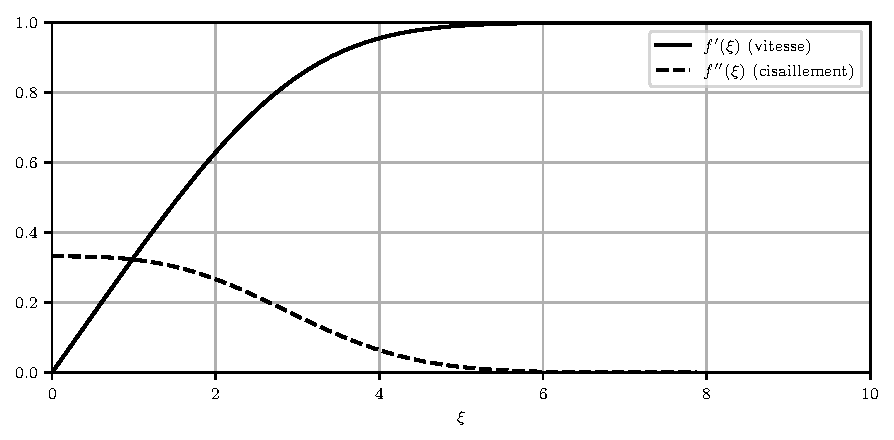
\includegraphics[scale=1]{mecaflu/blasius2.pdf}
    \vspace{-1em}
    \caption{Solution de l'équation de Blasius.}
\end{figure}
\end{EnvUplevel}
    \question En déduire un critère plus rigoureux pour l'épaisseur de la couche limite.
\end{questions}

\plusloin
Décrire qualitativement l'écoulement pour $x \gg \dfrac{\nu}{U_0}$ et faire un schéma représentant les deux régimes.

\newpage

\section{Forces d'inertie}
% Niveau :      PC
% Discipline :  Mécaflu
%Mots clés :    Viscosité, Couche limite, Equation de Blasius

\begin{exercise}{Anticyclones et dépressions}{3}{Spé}
{Mécanique des fluides, Mécanique en référentiel non galiléen, Fluide géostrophique}{bermu}

Le but de cet exercice est d'aborder la dynamique de l'atmosphère à la surface de la Terre à l'échelle globale. On se place dans le référentiel terrestre en rotation à la vitesse $\vOm = \Omega\ve_z$.

\DeclareNonDimensionalNumber{R}{o} %Rossby

\begin{questions}
    \questioncours Quelles sont les différences forces volumiques qui s'appliquent à un fluide à la surface de la Terre ? Exprimer notamment le terme d'inertie d'entraînement sous forme de potentiel.
    \question\label{que:rossby} En interprétant le nombre de Rossby 
    $$\RoN = \dfrac{v}{2L\Omega\cos\theta}$$
    et en l'estimant pour l'atmosphère, justifiez que l'équation de Navier--Stockes puisse se simplifier ainsi
    $$\pdv{\vv}{t} + 2\vOm\cross\vv = -\grad\qty(\dfrac{p}{\rho} + \Phi) + \nu\grad^2\vv,$$
    où $\Phi(r)$ est un potentiel dont on donnera la cause physique et l'expression.
    \question On s'intéresse aux courants géostrophiques qui sont de basse fréquence et de viscosité négligeable.
    \begin{parts}
        \part Quel est l'ordre de grandeur des fréquences concernées ?
        \part Justifier que la composante ascensionnelle de la vitesse ($v_r$) est négligeable.
        \part\label{que:buys} Montrer la loi de Buys--Ballot :
        
            \quad\begin{minipage}{15cm}
            \itshape i. Dans l'hémisphère nord, si on se place dos au vent, il y aura une dépression à notre gauche et un anticyclone à notre droite ; et inversement dans l'hémisphère sud. \\
            ii. En suivant ainsi le vent, il subira toujours la même pression.
            \end{minipage}
        \part Interpréter ces résultats sur les vents géostrophiques en termes météorologiques à l'aide de la figure ci dessous.
    \end{parts}
    \end{questions}
\begin{EnvUplevel}
\begin{figure}[H]
    \centering
    \vspace{-1em}
    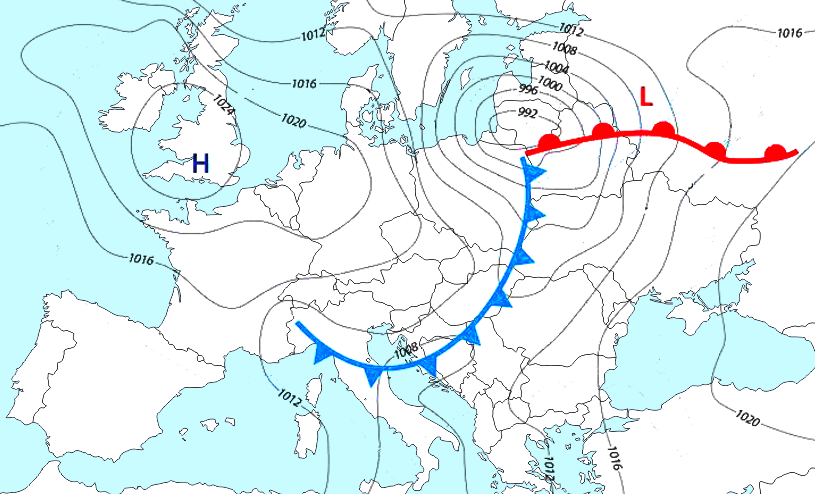
\includegraphics[width=0.9\linewidth]{mecaflu/meteo.png}
    \caption{Carte de fronts et d'isobares météo en Europe du 5 Juillet 2018.}
    \label{fig:my_label}
\end{figure}
\end{EnvUplevel}

\begin{center}
    \vspace{-1.5em}
    \itshape --- \quad Suite au verso \quad ---
\end{center}
\end{exercise}

\pagebreak

\printexerciseheader

\begin{center}
    \itshape --- \quad Suite du recto \quad ---
\end{center}

\bigskip

\begin{questions}
\setcounter{question}{3}
    \question On s'intéresse à présent aux effets de viscosité sur les vents géostrophiques. Pour simplifier, on va supposer que nous sommes en Europe où la latitude est environ de 45$^\circ$ N.
    \begin{parts}
        \part Estimer la valeur du nombre de Reynolds $\ReN$. Dans quelles régions les effets visqueux vont être prédominants ?
        \part Considérant que nous sommes en 2D et en utilisant le résultat \emph{ii.} de la question \ref{que:buys}, projeter l'équation précédente suivant les isobares horizontales et dans la direction perpendiculaire.
        \part Par un changement de variable complexe, monter que la viscosité à pour effet que la vitesse au sol fait un angle à 45$^\circ$ (sans rapport avec la latitude) par rapport aux isobares et qu'elle s'oriente vers ces dernières avec l'altitude en faisant une spirale.
        \part Donner l'altitude caractéristique $\delta$ de cette couche visqueuse et conclure par rapport au cas précédent.
    \end{parts}
\end{questions}

\plusloin
Il existe également des phénomènes ondulatoires appelés ondes inertielles que l'on peut déduire de l'équation de la question \ref{que:rossby}.

En outre les phénomènes météorologiques sont étroitement liés à la convection thermique entre les zones équatoriales où il fait chaud et les zones polaires où il fait froid.
% Niveau :      PC
% Discipline :  Mécaflu
%Mots clés :    Viscosité, Couche limite, Equation de Blasius

\begin{exercise}{\'Equation des marées de Laplace}{4}{Spé}
{Mécanique des fluides, Mécanique en référentiel non galiléen, Fluide géostrophique}{bermu}

Le but de cet exercice est d'aborder le mouvement des océans à la surface de la Terre à l'échelle globale et l'effet des marées. On se place dans le référentiel terrestre en rotation à la vitesse $\vOm = \Omega\ve_z$. On se place en coordonnées sphériques colatitude $\theta\in\qty[0,\pi]$ -- longitude $\varphi\in\qty[0,2\pi]$.

\DeclareNonDimensionalNumber{R}{o} %Rossby

\begin{questions}
    \questioncours Quelles sont les différences forces volumiques qui s'appliquent à un fluide à la surface de la Terre ? Exprimer notamment le terme de pesanteur sous forme d'un potentiel $\Phi(\vr)$ dont on donnera l'expression.
    \question En estimant la valeur du nombre de Reynolds $\ReN$ et du nombre de Rossby
    $$\RoN = \dfrac{v}{2L\Omega\cos\theta},$$
    justifiez que l'équation de Navier--Stockes puisse se simplifer ainsi
    $$\pdv{\vv}{t} + 2\vOm\cross\vv = -\grad P, \qquad P = \dfrac{p}{\rho} + \Phi(r) + \varphi(\theta,\phi),$$
    où $\Phi(r)$ et $\varphi(\theta,\phi)$ sont des potentiels dont on donnera la cause physique.
\begin{EnvUplevel}
On considère que la Terre est une sphère de rayon $R$ sur laquelle en l'absence de forces de marées il y a une hauteur $H$ d'océans. On appelle $\zeta(\theta,\phi,t)$ la hauteur de la mer par rapport à l'équilibre telle que
$$v_r|_{r = R + H} = \pdv{\zeta}{t}.$$ 
\end{EnvUplevel}
    \question En justifiant que le terme potentiel vertical est négligeable
    $\displaystyle\pdv{P}{r} \simeq 0$, montrer que le potentiel de pression puisse s'écrire
    $$P \simeq \dfrac{p_\text{atm}}{\rho} + g\zeta + \varphi.$$
    \question En utilisant l'incompressibilité du fluide (pour l'éq.~\ref{eq:laplace1}) et en justifiant les approximations qui vous sembleront pertinentes, déduire le système d'équation suivant, dit équations des marées de Laplace
    \begin{align}
    \pdv{\zeta}{t} &= -\dfrac{H}{R\sin\theta}\qty[\pdv{}{\theta}\qty(\sin\theta v_\theta) + \pdv{v_\phi}{\phi}] \label{eq:laplace1} \\
    \pdv{v_\theta}{t} - 2\Omega\cos\theta v_\phi &= -\dfrac{1}{R}\qty[g\pdv{\zeta}{\theta} +\pdv{\varphi}{\theta}], \\
    \pdv{v_\phi}{t} + 2\Omega\cos\theta v_\theta &= -\dfrac{1}{R\sin\theta}\qty[g\pdv{\zeta}{\phi}+\pdv{\varphi}{\phi}].
\end{align}
\end{questions}

\paragraph{Données :} en coordonées sphériques
\begin{align*}
    \vr = r\ve_r &= r\cos\theta\ve_z + r\sin\theta\sin\phi\ve_x + r\sin\theta\cos\phi\ve_y \\
    \grad P &= \pdv{P}{r}\ve_r + \dfrac{1}{r}\pdv{P}{\theta}\ve_\theta + \dfrac{1}{r\sin\theta}\pdv{P}{\phi}\ve_\varphi \\
    \div\vv &= \dfrac{1}{r^2}\pdv{r^2 v_r}{r} +  \dfrac{1}{r\sin\theta}\pdv{}{\theta}\qty(\sin\theta v_\theta) + \dfrac{1}{r\sin\theta} \pdv{v_\phi}{\phi},
\end{align*}

\end{exercise}

\section{Bilans macroscopiques}